\documentclass[12pt]{article}

\usepackage[margin=1in]{geometry}
\usepackage{graphicx}
\usepackage{hyperref}
\usepackage{listings}

\title{EagerDB:\\
A Predictive Cache Warming Tool\\
6.885 Final Paper
}

\author{
John J. Wang\\
wangjohn@mit.edu\\
}
\date{\today}

\begin{document}
\maketitle

\abstract{
Many applications increase database performance using some form of caching. The majority of cache implementations, however, only increase performance for queries that have been already seen. EagerDB takes this a step farther and provides a predictive cache. It predicts queries that will occur in the future with high probability and automatically loads them into the cache. EagerDB allows the user to manually specify query preloads or automatically parse historical database logs, estimate a Markov model, and preload queries which have high transition probabilities.
}

\section{Introduction}

Most web applications improve database performance by caching -- storing data has previously been used. Using a cache can dramatically improve database performance when temporal locality is present (i.e. when previously requested data is requested multiple times). Caching has become one of the most fundamental concepts in computer science, and in turn, almost all large technology companies use caches in some form.

However, caches assume that historical data repeats. This assumption does not capture all of the potential performance gains that are possible. In fact, there is quite a large amount of data that exists which can be used to improve performance even further. Since there workflows of users tend to be methodical, the queries that get sent to a database can be predicted. One can then estimate the probability of some query $X$ happening given the current state of the database, and ``preload'' $X$ when it has a high probability of happening.

EagerDB provides a framework for preloading such queries. Developers can manually specify queries to preload or they can use a prediction engine for discovering queries to preload. EagerDB is built as a Ruby gem and can be easily included in a Ruby on Rails web application for easy improvements in database performance. This paper shall outline the design of EagerDB, the reasons for making particular design decisions, and the results of benchmark tests.

\section{Background}

There have been a number of papers which have thought to use predictive caching. Lempel and Moran (2003) use predictive caching to improve the speed of search results. However, their prefetching is entirely specific to search, and they focus their attention on the optimal number of pagesof search results, $n$, to prefetch into an in-memory cache. Although Lempel and Moran (2003) make a leap of forward progress for predictive caching, they do not solve the general problem of predictive caching for arbitrary query types.

Kraiss and Weikum (1998) use a Markov model for predictive caching in the context of multimedia document archives. In their work, documents are speculatively prefetched if the expected number of hits on a document is higher than the expected number of hits on the documents that must be dropped from the cache. Unfortunately, this framework does not account for the complexity of database queries. Although the number of documents in an archive is finite, the number of possible queries to a database is infinite.

EagerDB extends the idea of predictive caching to be more general. In essence, any query that is sent to a database can be a predictor for a future query. The future query, moreover, can be correlated with the original query. EagerDB provides a flexible framework for defining relationships between a query being sent to the database and future queries.

\section{Manual Query Syntax}

EagerDB has its own easy to use syntax for manually specifying preloads. Behind this manual query syntax is the idea that any query $Y$ can be used as an indicator for a later query $X$. Thus, if the probability of $X$ occurring is high given that $Y$ has occurred, then one should preload $X$ by bringing it into the database's cache. We call $Y$ the \emph{match statement}, and $X$ the \emph{preload statement}.

\subsection{Basic Definitions}

In order to explain match and preload statements more, we need to make a distinction between non-binded and binded SQL queries. A \emph{binded SQL query} is just any instance of a valid SQL statement which contains table, column, and attribute values. An example of a binded SQL query would be:

\begin{lstlisting}
SELECT * FROM distributors WHERE name = 'walmart' AND
  town = 'Chicago' AND state = 'IL'
\end{lstlisting}

A \emph{non-binded SQL query} is just an instance of a valid SQL statement which contains table and column values, but does not contain attribute values. For example, the non-binded version of the previous SQL query would be:

\begin{lstlisting}
SELECT * FROM distributors WHERE name = ? AND
  town = ? AND state = ?
\end{lstlisting}

Non-binded SQL queries can be converted into binded SQL queries by providing \emph{bind values}, an array of values which would be inserted into each bind location (denoted by a $?$ in the non-binded SQL query). To convert the previous non-binded SQL statement into a binded SQL statement, one would need to pass in the following array of bind values:

\begin{lstlisting}
['walmart', 'IL']
\end{lstlisting}

\subsection{Match Preload Files}

Match and preload statements are non-binded SQL queries. Match statements allow EagerDB to match on a particular SQL statement structure, and preload statements allow us to preload a specific SQL statement structure when match statements occur. In this vein, one could manually specify match and preload statements. This is done by first specifying a single match statement, then any number of preload statements to load into the cache whenever that match statement is seen.

In a \emph{match preload file} (MP file), a developer using EagerDB can specify a list of match statements and their corresponding preload statements. EagerDB can read over an MP file and incorporate any match and preload statements that have been made inside the file. A developer can use the MP file as a stand-alone product without running the Markov model so that the preload statements in the MP file will be the only statements preloaded by EagerDB, or incorporate the MP file as an addition on top of the Markov model's statements. The syntax for an MP file is straightforward:

\begin{itemize}
  \item Match statements are preceded by a dash ``-''.
  \item Preload statements are preceded by a rocket ``=\textgreater''. Preload statements will be paired with the last match statement seen in the MP file.
  \item SQL statements are encapsulated by quotation marks.
  \item Bind values, separated by commas, follow the SQL statement. The $i^{\textrm{th}}$ bind value in the SQL statement corresponds to the $i^{\textrm{th}}$ comma separated value after the SQL statement.
\end{itemize}

In addition to these syntax rules, there are methods provided for bind values which allow making general preload statements much easier. We provide the \texttt{match\_result} and \texttt{match\_bind\_value} keywords.

The \texttt{match\_result} keyword provides access to the result of the match statement of a preload. One can access the value of a column in the result by asking for the column name like so: \texttt{match\_result.column\_name}. For example, if a developer wanted to access the id of the result from his match statement, he could write a preload statement like so:

\begin{lstlisting}
=> "SELECT * FROM things WHERE product_id = ?", match_result.id
\end{lstlisting}

The \texttt{match\_bind\_value} keyword is a similar construction, but provides access to the bind value of the binded instance of the match statement. One specifies an index $i$ after the \texttt{match\_bind\_value} keyword, which gives access to the $i$th bind value from the match statement. For example, one could write:

\begin{lstlisting}
- "SELECT * FROM products WHERE name = ?"
  => "SELECT * FROM things WHERE product_name = ?", match_bind_value(0)
\end{lstlisting}

In the above, whenever of a SQL query of the form \texttt{SELECT * FROM products WHERE name = ?} is seen, EagerDB will take the zeroth bind value (bind values are indexed by 0) from the statement and use it as the zeroth bind value in the preload statement \texttt{SELECT * FROM things WHERE product\_name = ?}.

\begin{figure}[h]
\begin{lstlisting}[frame=single]
- "SELECT * FROM users WHERE name = ?"
  => "SELECT * FROM products WHERE owner_id = ?",
      match_result.id

- "SELECT * FROM pinterest WHERE pin = ? AND interest = ?"
  => "SELECT * FROM tables WHERE pin = ? AND interest = ?",
      match_bind_value(0), match_bind_value(1)
  => "SELECT * FROM interests WHERE interest = ? AND
      pinterest_id = ?", match_bind_value(1), match_result.id
\end{lstlisting}
  \caption{\label{fig:mp-file-example}A snippet from an MP file}
\end{figure}

Figure \ref{fig:mp-file-example} provides an example instance of an MP file. In this file, there are two match statements. The first match statement has a single preload, while the second match statement has two preloads. EagerDB will listen to the stream of SQL queries coming from the database, and whenever a match statement matches the structure of a query, the preload statements associated with that match statement will be brought into the database's cache.

For example, using the MP file from figure \ref{fig:mp-file-example}, suppose the following sequence of queries arrived at the database (ordered chronologically):

\begin{lstlisting}
SELECT * FROM products WHERE name = 'table' AND state = 'IL'
SELECT * FROM users WHERE name = 'john'
SELECT * FROM laptops WHERE BRAND = 'lenovo' AND serial_number = '5'
\end{lstlisting}

Then, after the second query (\texttt{SELECT * FROM users WHERE name = 'john'}) was run, its corresponding preload statement would be brought into the cache. For example, if the second query returned a result with an id of 52, then the following query would be brought into the database's cache: \texttt{SELECT * FROM products WHERE owner\_id = 52}. The other queries in the sequence did not match the structure of any of the match statements, so EagerDB would not bring anything into the cache after their execution.

\section{System Design}

The EagerDB system is designed to be as unobstrusive as possible. It sits at the middleware level and only needs two things: 1) a connection to the stream of SQL queries and results being sent to and from the database and 2) a connection to the database for preloading queries. As a Ruby gem, EagerDB requires a minimal amount of integration and can be incorporated into a Ruby on Rails web application with less than 15 lines of code.

The system is also designed to be distributed and scalable. The EagerDB system is easily extended to multiple machines and can still be used with a sharded database. More details of the design later in the paper will show how this can be accomplished without any changes to the framework.

EagerDB is designed for flexibility, since it works on any database with a built-in cache, including MySQL, PostgreSQL, etc. It is SQL syntax agnostic, meaning that small variations in the syntax between different databases will not prevent EagerDB from preloading queries. This quality comes about because of the non-binded vs. binded SQL abstraction: all match statements are non-binded and general. In fact, EagerDB could potentially preload NoSQL queries, such as those from MongoDB, without any problems.

Additionally, EagerDB uses the database's own cache. This greatly simplifies setup and reduces the number of failure points. Instead of providing its own cache, which would have to deal with cache invalidation issues as well as duplication of data, EagerDB can rely on the pre-built mechanisms of the database. Thus, the design is resistant to bloating memory, and a user can tweak the size and properties of a single cache (instead of two). Moreover, using the database's own cache means that EagerDB can be used on more than just web applications. Since it has no appliction-specific logic, EagerDB can be used for anything that sends sends queries to a database.

Finally, EagerDB internally reads data from the MP file format, which enables a developer to change automatically generated preloads and provide their own preloads relatively easily. Having a single format for representing data greatly simplifies the amount of work a developer needs to do to make changes to their own preloads.

In order to accomplish all of the above traits, EagerDB makes a number of abstractions which will be presented in this section. The codebase is written in Ruby (so that it can conveniently be used in Ruby on Rails web applications) and is broken up into two sections. The first is the processing code, which provides the infrastructure for parsing MP files and running EagerDB with a live stream of queries, and the second is the prediction code, which creates a Markov model and outputs an MP file based on historical database logs.

\subsection{Processing Code}

The processing code provides abstractions for listening to a stream of queries going to the database, encapsulating each query as a job to be processed, and finally processing those jobs and sending the resulting preload queries (if there are any) back to the database to be executed. When the preload queries get to the database, they will warm the database's cache and will speed up the execution of the same query in the future. Figure \ref{fig:system-overview} provides an overview of the high-level architecture.

\begin{figure}[h]
  \centering
  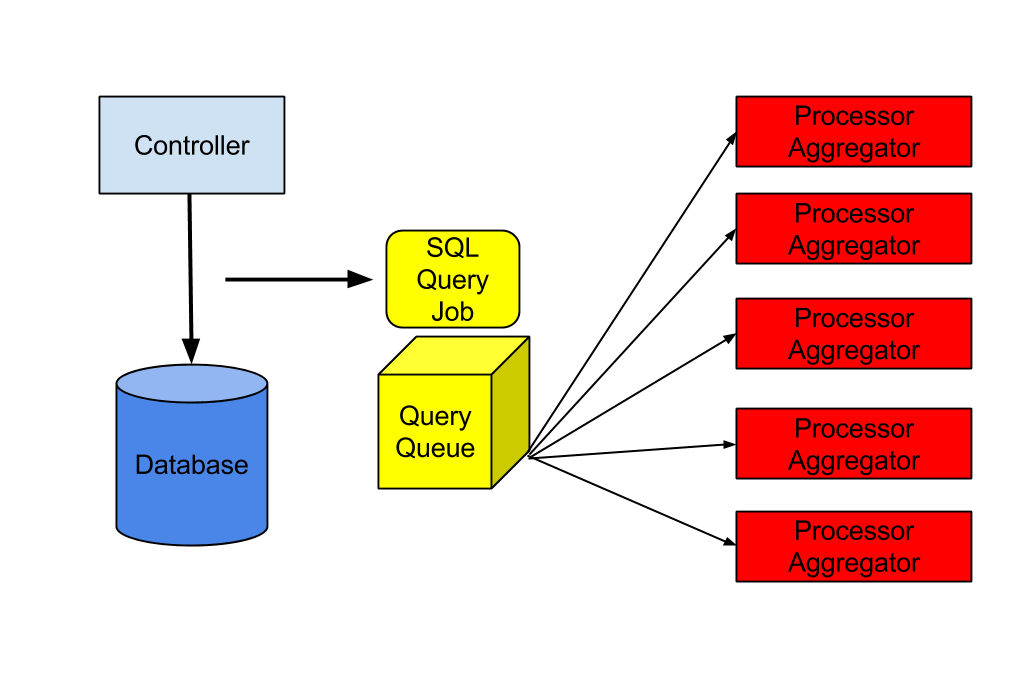
\includegraphics[width=4in]{figures/eager_db_overview.png}
  \caption{\label{fig:system-overview}SqlQueryJobs are created from the incoming stream of queries, placed onto a queue, and finally sent to processor aggregators.}
\end{figure}

First, a \texttt{CommunicationChannel} object sits between the database and the controller and listens to queries that get sent to the database. Whenever a query appears in the \texttt{CommunicationChannel}, the query and its result will be processed and converted into a \texttt{SQLQueryJob}. This job is then placed on a query queue, which temporarily holds the \texttt{SQLQueryJob}s. A process runs and attempts to keep the query queue empty at all times, sending \texttt{SQLQueryJob}s as quickly as possible to an instance of a processor aggregator. Each processor aggregator will handle a \texttt{SQLQueryJob} and determine which preload statements (if any) need to be sent to the database.

Processor aggregators hold the many processors, the fundametal object for computation in EagerDB. Processors hold a single match statement and multiple preload statements. The processor is an encapsulation of a match statement and its preloads as defined in an MP file. There are two crucial methods for a processor in its public API, these are \texttt{matches?} and \texttt{process\_preloads}. The \texttt{matches?} method takes in a raw, binded SQL query from the \texttt{SQLQueryJob} (originally part of the stream of SQL queries going to the database) and checks if that query matches the processor's match statement. The \texttt{process\_preloads} method will take in the same raw, binded SQL query, and will return binded preloaded statements if \texttt{matches?} returns true, and an empty list otherwise.

Each processor aggregator holds all of the processors from an MP file, and all processor aggregators are equivalent. When used with a single machine, EagerDB would only create a single processor aggregator, but one could create many more processor aggregators to scale. Figure \ref{fig:processor-aggregator} shows an overview of the processor aggregator. Basically, the aggregator parses the raw SQL from the \texttt{SQLQueryJob}, then hands off the resulting job to the correct processor. If the parsed SQL matches a processor's match statement, then that processor's preload statements get added to the preload query queue, and will eventually reach and be executed by the database.

\begin{figure}[h]
  \centering
  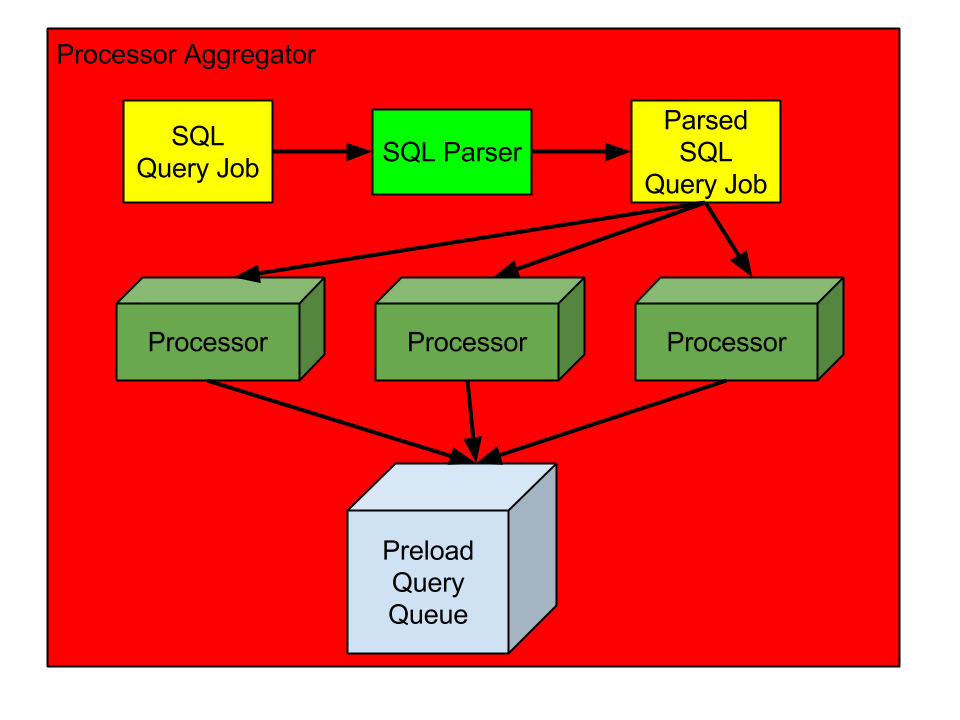
\includegraphics[width=3in]{figures/processor_aggregator.png}
  \caption{\label{fig:processor-aggregator}Processor aggregators process the SqlQueryJob (which contains raw, non-binded SQL from the stream) and sends parsed result to individual processors. Matches result in preloads getting sent to a preload queue.}
\end{figure}

The default implementation of the query processor uses a hash table so that statements can be matched very quickly. When a new \texttt{SQLQueryJob} comes in, the non-binded SQL is used as a key in the hash table. The hash table values for a particular non-binded SQL key is an array of all processors that match on that SQL statement. Thus, the total time required to process any statement and load preloads is $O(k)$ where $k$ is the number of matching statements (assuming that the number of preloads per match statement is less than some constant). Most applications tend to have incredibly small $k$'s, which makes this process extremely fast. This runtime is also asymptotically optimal because loading a match statement's $k$ preloads will require $\Omega(k)$ runtime.

\subsection{Sharding Databases and Scaling EagerDB}

This subsection will spend some time discussing implications of design decisions on scaling. First, notice that increasing throughput for EagerDB jobs is incredibly easy: just add more processor aggregators. We have a couple nice properties that allow this to occur. First, each \texttt{SQLQueryJob} only needs to go to a single processor, since each aggregator is identical. Second, \texttt{SQLQueryJob}s can be dropped by the network without fear of losing real information (only possible performance improvements). Of course, if the probability of a network failure is $p$, and the developer wanted an arrival rate of $a$, then one could send $\lceil a/p \rceil$ \texttt{SQLQueryJob}s over the network to obtain the required arrival rate.

Sharding the underlying database is also quite easy, as long as an appropriate function for mapping a SQL query to a particular shard exists. Each database shard would get its own query queue. The query queue would have access to all processor aggregators, and the processor aggregators would have references to all database shards. The preload query queue on each processor aggregator would send the preload query to the correct shard by invoking the function for mapping queries to shards. Thus, sharding databases, though not implemented in the current version of EagerDB, can be performed without major modifications to the underlying framework.

\subsection{Prediction Code}

This section will discuss how automatic prediction of high probability preloads are made. The general idea is to build a Markov model based on historical database logs, then find match-preload pairs with high transition probabilities. We think of the state of the Markov model at time $t$ as the last raw, binded SQL query that was run before time $t$. Thus, we want to find an estimate of $P(X | Y)$ for all $X$ in the set of possible queries and where $Y$ is the current state. We can then create a match pair if $P(X | Y) > \lambda$ for some parameter $\lambda$. A match pair, denoted as $(Y, X)$, are two non-binded SQL statements, where $Y$ is the match statement and $X$ is the preload statement.

To estimate $P(X | Y)$, we will use historical database logs and a time parameter $T$. Here, $T$ will be a time after which queries are no longer considered pairs. For example if $Y$ occurs, then $X$ occurs 10 years later, there is a very little chance that $Y$ is actually predictive of $X$. Thus, we will only consider $(Y, X)$ pairs where $X$ occurs within time $T$ after $Y$ has occurred. The complete algorithm for estimating probability is as follows:

\begin{itemize}
  \item Break apart and group database logs by user id or ip-address (or a similar metric, depending on which is available in the data). Each group should contain the queries made by a single user or ip-address.
  \item For each query $Y$ in the group, find the other queries $X$ which occur within time $T$ of $Y$ occurring, and increment the count, $C((Y,X))$, of the $(Y,X)$ pair. Also, increment the count, $C(Y)$, of the number of times $Y$ occurs.
  \item After processing each group, and all queries in each group, you have the total occurrences of each $(Y,X)$ pair, and the total occurrences of each query $Y$. Now use the estimate $\hat{P}(X | Y) = C((Y,X))/C(Y)$. Check if $\hat{P}(X | Y) > \lambda$ for any $Y, X$ pair. Return all such $(Y, X)$ pairs as a match.
\end{itemize}

Notice that this calculation is easily parallelizable in the MapReduce framework. The grouped queries for a particular user or ip-address are passed as documents in the map step, where each document contains queries for a particular user or ip-address. Then, for each query $Y$, we can emit the $Y$ as the key, and an array of all the $X$'s which occur within $T$ time of $Y$ occuring as the value. In the reduce step, we compute $\hat{P}(X | Y)$ for all possible $X$'s that have been sent to this particular node. We do this by computing $C((Y,X))$ and $C(Y)$, since we can record a count of the total number of times $Y$ occurred, as well as the number of times $X$ occurs in the array of values. In this way, massive database logs can be broken up and used for finding potential match pairs.

Now we have identified pairs of queries which happen together with high probability. More specifically, we can say that if $Y$ occurs, then $X$ occurs with high probability within $T$ after $Y$ occurs. We now need to identify the bind values for $X$. To do this, we can look through all of the binded, raw occurrences of $Y$ (i.e. the raw SQL query going to the database), identify its bind values, and compare them to all of the subsequent binded $X$ occurrences. We can then find a mapping between the bind values indices on $Y$ and $X$, and see if this mapping persists across all $X$'s. For example, consider the following match pair (in MP file syntax):

\begin{lstlisting}
- "SELECT * FROM names WHERE name = ?"
  => "SELECT * FROM hats WHERE owner = ?"
\end{lstlisting}

If there were many example instances of this rule, and it happened that the zeroth bind value in the match statement (``name = ?'' in the above example) was the same as the zeroth bind value in the preload statement (``owner = ?'' in the above example) with high probability, then one could expect the bind value in the preload statement to be \texttt{match\_bind\_value(0)}. EagerDB uses a probabilistic algorithm similar to this for finding bind values in preloads. For bind values requiring the use of \texttt{match\_result}, EagerDB uses a best guess and performs fuzzy matching on the result's column name, and the bind value's column name. For example, in the above example, if the result of the match query returned rows with a column attribute named ``owner'', then EagerDB would use \texttt{match\_result.owner} as the bind value.

\section{Results}

To test the performance of EagerDB, we ran benchmark tests using MySQL version 5.5.34, for debian-linux-gnu. We chose to use the OLTP database benchmark suite, which can be found at \url{http://www.oltpbenchmark.com}. In particular, we focused on the Twitter benchmark, which simulates a workload similar to the one that would be received by Twitter databases. We modified the performance benchmark slightly, removing all inserts (since EagerDB does not handle insertions) and adding a Markov model so that it had transition probabilities between states.

The Twitter benchmark was chosen due to its simplicity (a small number of tables and attributes). Because it is not as complex as other benchmarks (the TPCC benchmark for example) the Twitter benchmark can be used to gain intuition for how well EagerDB performs. The modified Twitter benchmark had four tables with the following attributes:

\begin{itemize}
  \item \texttt{user\_profiles}: INT id, CHAR(20) name
  \item \texttt{tweets}: INT uid, CHAR(20) name, VARCHAR(200) data
  \item \texttt{follows}: INT f1, INT f2
  \item \texttt{followers}: INT f1, INT f2
\end{itemize}

The \texttt{tweets} table has a foreign key \texttt{uid} into the \texttt{user\_profiles} table. Additionally, \texttt{f1} and \texttt{f2} are both foreign keys into the \texttt{user\_profiles} table for both the \texttt{follows} and \texttt{followers} table. We created a Markov process which had some probability of making a completely random query with randomly chosen bind values. It also had some probability of making a child query, which used the result and bind values of the previous query to make a new query. The intuition behind this Markov process is that when $a$ navigates to $b$'s profile on twitter, there is some probability that $a$ will click to find all of $b$'s followers or that $a$ will click to find out who $b$ is following. Figure \ref{fig:queries-simulated} shows the query types that were simulated.

\begin{figure}[h]
\begin{lstlisting}[frame=single]
GetTweets:    "SELECT * FROM tweets WHERE uid = ?"
GetFollows:   "SELECT f2 FROM follows WHERE f1 = ? LIMIT 20"
GetFollowers: "SELECT f2 FROM followers WHERE f1 = ? LIMIT 20"
\end{lstlisting}
\caption{\label{fig:queries-simulated}Simulated Queries in Modified Twitter Benchmark}
\end{figure}

The Markov process was structured as follows:
\begin{itemize}
  \item \texttt{GetTweets} queries could have child queries of \texttt{GetFollows} or \texttt{GetFollowers}, where \texttt{f1} would be equal to the \texttt{uid} from \texttt{GetTweets}.
  \item \texttt{GetFollows} queries could have a child query of \texttt{GetTweets}, where \texttt{uid} would be randomly selected from \texttt{f2} in the result of the \texttt{GetFollows} query.
  \item \texttt{GetFollowers} queries could have a child query of \texttt{GetTweets}, where \texttt{uid} would be randomly selected from \texttt{f2} in the result of the \texttt{GetFollowers} query.
\end{itemize}

We populated a database with 100 users, 5000 tweets, 2000 follower relationships, and 2000 follow relationships. Then, we ran performance tests with and without EagerDB, using different probabilities for navigating to a child query. Table \ref{fig:performance-results} shows the results of our tests.

We ran the tests for varying child query probabilities. We define the child query probability $p$, as the probability that the Markov process will navigate to a child query using the previous query. The probability of creating a completely random query is then $1-p$.

\begin{table}[h]
  \centering
  \begin{tabular}{c | c c c }
    & \multicolumn{3}{c}{\large Query Type} \\
                Child Query &                 &                 & \\
                Probability & GetFollows      & GetFollowers    & GetTweets \\
    \hline \hline
                  $p = 0.1$ & \textbf{8.34\%} & \textbf{4.83\%} & \textbf{4.99\%} \\
                            & \textbf{(7.29)} & \textbf{(5.08)} & \textbf{(5.53)} \\
    \\
                  $p = 0.2$ & 0.46\%          & 27.3\%          & 14.3\% \\
                            & (0.43)          & (1.01)          & (1.26) \\
    \\
                  $p = 0.3$ & 18.9\%          & 1.89\%          & \textbf{39.5\%} \\
                            & (1.27)          & (0.98)          & \textbf{(1.83)} \\
    \\
                  $p = 0.4$ & \textbf{8.09\%} & \textbf{36.1\%} & \textbf{35.1\%} \\
                            & \textbf{(7.78)} & \textbf{(1.74)} & \textbf{(1.68)}
  \end{tabular}
  \caption{\label{fig:performance-results}Performance Results: Percentage improvement in latency when running Twitter benchmark with and without EagerDB. Positive numbers indicate EagerDB has decreased average latency. Numbers in parentheses are t-statistics, and bolded text connotes statistical significance at the 95\% level.}
\end{table}

Table \ref{fig:performance-results} shows the results of running the Twitter benchmark with and without EagerDB. The table shows percentage improvements in average latency using EagerDB. In the table, one can see that overall, EagerDB improves performance significantly for different types of queries. As the probability $p$ of transitioning to a child query increases, we tend to see an increase in the magnitude of the performance improvement. This observation makes intuitive sense because as the probability of going to a random query goes down, it is more likely that the match-preload statements in EagerDB will be predictive of future queries.

Thus, EagerDB improves performance across the board for the Twitter benchmark. There are no types of queries (with any probability $p$), where one does not see a nominal performance improvement (although some are not statistically significant). This provides strong evidence that EagerDB improves performance, at least for workloads which have some non-zero probability of using previous query bind values or results. The results in table \ref{fig:performance-results} seem to suggest that EagerDB can improve performance in applications where each user has a predefined, methodical workflow.

Another observation from the benchmark results was the ease of integration. Only 9 lines of code were needed in order to fully integrate EagerDB into the Twitter Benchmark. Since EagerDB is both easy to integrate and performant, one can improve database speed without much effort.

A final observation to make on the result data alludes to a potential optimization for the future. There were some cases where the variance in the latencies for queries was quite high when the benchmark was run with EagerDB. In fact, looking at the underlying data, one could consistently see that about 0.2\% to 0.5\% of queries were three or more standard deviations above the mean when using EagerDB. However, the benchmark without EagerDB never had these types of outliers. Thus, there were a small number of times when EagerDB caused excessively long query latencies. This is potentially due to the fact that a query would arrive at the database while its preload query was being cached. Thus, the query would have to wait for the preload to finish before executing, causing much longer query latency. To avoid this, EagerDB in the future should implement a stop protocol that prevents a preload statement from executing after a particular expiration time.

\section{Conclusion}

This paper presented EagerDB, a predictive cache warmer for database queries. EagerDB sets out to improve performance by using historical database logs to predict future queries. The design of EagerDB makes it scalable, flexbile, and easily configured to many applications. In particular, the design enables distribution of processor aggregators across multiple machines, sharding on the underlying database, easy integration into applications, and parallelized processing of historical database logs.

All of these serve to increase the performance of a database-backed application while minimizing the amount of setup time required. EagerDB can be used to help optimize many web applications which have repetitive workflows, where database queries will not necessarily be cached.

There are many future directions for research. First, EagerDB was actually designed so that processors could be subclassed, so that developers could write their own processors. For example, one might want to match on more than just a single query, or use application meta-data in order to help preload queries. One can currently write such a processor, but there is no way to include such metadata. A small step towards this more flexible framework would be to include application-level metadata in \texttt{SQLQueryJob}s.

Next, the system should begin to optimize how raw SQL and the results from the raw SQL query get sent to processors. Currently, the results and the raw SQL are both encapsulated with a \texttt{SQLQueryJob}, then sent to a processor aggregator. However, executing the SQL query and waiting for the results causes extra wait time before the \texttt{SQLQueryJob} can be sent to its processor aggregator (sometimes a couple hundred milliseconds). An improvement would be to have the raw SQL sent in a \texttt{SQLQueryJob} immediately to a processor aggregator. While the aggregator processes this job, the result of the query could be placed in a staging area where processed preloads are sent. After the result and its corresponding preloads are both in the staging area, the preloads could inject the correct bind values using the result and be sent off to be executed by the database.

EagerDB is a step towards automatically improving database performance. This paper has described its design and shown its proficiency in handling repetitive workflows.

\end{document}
